\Chapter{RESULTATS NUMÉRIQUES}\label{sec:Theme3}
\section{Outils de comparaison}\label{sec:out}
Les premières recherches visant à comparer les performances de solveurs sur un problème unique ou une série de problème utilisaient des métriques facilement quantifiables telles que le nombre d'appels à la fonction~\cite{BoCoGoTo1995} ainsi que le temps de résolution en secondes~\cite{Mi99}. Cependant, ces indicateurs sont moins appropriés en situation de résolution d'un grand nombre de problèmes. Puisque ces métriques sont spécifiques à un problème, le banc d'essai qui incorpore chacune d'entre-elles prends des proportions énormes. Dans cet ordre d'esprit, certains outils ont été développés pour analyser une série de problèmes test, avec des dimensions et des spécificités différentes, sans qu'il en devienne laborieux d'en tirer des conclusions.
\subsection{Test et graphe de convergence}\label{sec:con}
Pour comparer la performance d'un ensemble d'algorithmes sur un seul problème, on aura recours au graphe de convergence. On y trace la courbe de la meilleure valeur de la fonction objectif obtenue en fonction du nombre d'appel à la fonction objectifs.

En optimisation sans-dérivées, contrairement à  en optimisation classique, rien n'assure qu'un solveur arrivera à l'optimum global, ou encore qu'un optimum soit atteint dans le budget alloué. De plus, en situation de résolution de boîte noire, il est impossible de connaître l'optimum théorique du problème, et ce si celui-ci existe. On aimerait tout de même quantifier la performance d'un solveur.  À cette fin, il est entendu dans la littérature de faire appel à un test de convergence qui mesure la capacité à l'algorithme à s'approcher de la meilleure solution obtenue par l'ensemble des algorithmes à l'étude, soit 
\begin{equation*}
f(x^0) - f(x) \geq (1-\tau)(f(x^0)-f^*)
\end{equation*}
issu de~\cite{MaNo02a} avec $x^0$ le point initial, $x$ le point courant, $f$ la fonction objectif, $\tau\geq0$ un seuil de tolérance et $f^*$ la meilleure solution courante trouvée par un des solveurs comparés sur ce problème. Le test de convergence peut être utilisé pour savoir si un solveur atteint au moins une solution proche de la meilleure en utilisant un $\tau$ grossier, par exemple $\tau = 0.1$, ou encore pour savoir si le solveur est capable d'obtenir $f^*$ en utilisant $\tau =0$. Il est possible que le test ne soit jamais réussi si on observe la résolution avec un budget d'évaluation fixe, ce qui sera nécessaire pour des boîtes noires bruitées, pour lesquelles la convergence de l'algorithme n'est pas assurée.

En situation de barrière progressive, le test de convergence doit être adapté pour tenir compte de l'impertinence de $f(x)$ pour $x\notin \Omega$. Afin de comparer seulement des points réalisables, on utilisera le test
\begin{equation*}
\bar{f}_{\textsf{fea}} - f(x_e) \geq(1-\tau)(\bar{f}_{\textsf{fea}}-f^*).
\end{equation*}
issu de~\cite{AuTr17}. $\bar{f}_{\textsf{fea}}$ y représente la valeur moyenne des premiers points réalisables obtenus dans les résolutions des différentes instances du même problème et $f(x_e)$ le meilleure valeur de la fonction objectif obtenue à un point réalisable.
\subsection{Profil de performance}\label{sec:pdp}
Un outil établi pour la comparaison de solveurs d'optimisation classique est le profil de performance~\cite{DoMo02}. La performance est donnée par une mesure $t_{p,s}$, qui peut être par exemple le nombre d'évaluations nécessaire pour l'obtention du minimal global, pour une paire de $p$ et $s$, un problème et un solveur. En optimisation sans-dérivées, on choisira le nombre d'itérations nécessaire à la satisfaction du test de convergence énoncé précédemment. Afin de comparer les solveurs sur chaque problème, on défini le ratio de comparaison suivant
\begin{equation*}
r_{p,s}=\frac{t_{p,s}}{\min\{t_{p,s} : s\  \epsilon \  S\}}
\end{equation*}
On peut alors définir le profil de performance d'un solveur sur un ensemble de problème $P$ ainsi
\begin{equation*}
\rho_s(\alpha)=\frac{1}{|P|}\text{size}\{p\ \epsilon \ P : r_{p,s} \leq \alpha \}
\end{equation*}
Pour un $\alpha$, soit un indice de performance tel que le ratio de comparaison $r_{p,s}$, on peut savoir la proportion de problème que chaque solveur a su résoudre en se rapprochant à un facteur de $(1-\tau)$ de la meilleure solution trouvée par l'ensemble des solveurs. Le test de convergence varie selon la nature des problèmes à résoudre. On peut utiliser un profil de performance pour des outils d'optimisation avec dérivés avec un $t_{p,s}$ qui agit sur les informations de premier ordre de la fonction, tel que le nombre d'évaluations pour atteindre $x$ tel que $f'(x)=0$. Ainsi, $\rho_s(\tau)$ revient à être la probabilité que le ratio de performance $r_{p,s}$ du solveur $s$ soit à un facteur $\tau$ du meilleur ratio possible. La lacune principale des profils de performance consiste en l'incapacité du ratio utilisé de prendre en compte la dimension du problème.

Il est important de noter que les profils  de performance ont une faille tel qu'élaboré dans~\cite{GoSc2016}. Les auteurs concluent que l'utilisation de $f^*$ dans le test de convergence implique que la simple observation des courbes sur un graphe n'est pas suffisante pour classes les algorithmes. Puisque la comparaison se fait avec le nombre d'itérations minimal observé, il se peut que, lorsqu'on compare entre-eux deux solveurs qui n'ont pas performés en tant que meilleur, l'ordre apparent ne soit pas celui qu'on observerait si on éliminait du graphe les données du meilleur. On se doit alors d'utiliser un autre outil pour mesurer les performances des solveurs sur un ensemble de données.
\subsection{Profil de données}\label{sec:pdd}
Moré et Wild proposent~\cite{MoWi2009} une définition d'un profil de donnée, 
\begin{equation*}
d_s(\alpha)=\frac{1}{|P|}\text{size}\{p\ \epsilon \ P : \frac{t_{p,s}}{n_p+1} \leq \alpha \}\\
\end{equation*}
avec $t_p$ le nombre d'évaluations pour atteindre la convergence nécessité par le solveur $s$ sur le problème $p$. Le facteur $n_p+1$ est le nombre d'évaluations nécessaire pour le calcul de l'estimation finie d'un gradient pour un problème de taille $n_p$. Il est alors possible de mesurer la performance relative des solveurs comme une fonction du budget d'évaluations, sans la comparaison que le ratio de performance imposait. Ainsi, pour un $\alpha$, soit une quantité de $n+1$ évaluations de la fonction objectif, on peut savoir la proportion de problèmes que chaque solveur a su résoudre en se rapprochant à un facteur de $(1-\tau)$ de la meilleure solution trouvée par l'ensemble des solveurs. L'avantage des profils de données sur les profils de performance est qu'il est possible de quantifier la performance du meilleur algorithme, compte tenu que celui-ci n'est plus comparé à lui-même. La faille évoquée par Gould et Scott~\cite{GoSc2016} n'est pas applicable aux profils de données puisqu'ils ne nécessitent
\section{Problèmes test}\label{sec:pro}
La comparaison des stratégies se fait sur plusieurs ensembles de problèmes tests. En premier lieu, un ensemble de problèmes non-linéaires sans contraintes et sans bornes est décrit afin de caractériser le comportement des algorithmes opportunistes sur un large ensemble de problèmes. En deuxième lieu, un échantillon de problèmes avec des contraintes relaxables et quantifiables est décrit afin d'observer la performance des différentes versions de la stratégies opportuniste en situation de barrière progressive. Enfin, on décrit en détails des cas de problèmes d'ingénierie connus comme pouvant être résolus avec des outils d'optimisation sans-dérivées dans le but de déterminer si la stratégie opportuniste a le potentiel d'influer la résolution d'une boîte noire d'expression non analytique.
\subsection{Ensemble de problèmes Moré-Wild}\label{sec:mw}
L'échantillon de problèmes analytiques caractéristiques $\Pset$ utilisé est celui proposé par Moré et Wild~\cite{MoWi2009}. Cet ensemble de problèmes est fréquemment réutilisé dans la communauté~\cite{VaVi07,CuRoVi10,ZhCoSc10,CoLed2011,AdAuBeYa2014,,AuLedTr2014}, ce qui justifie son utilisation comme base de problème analytique pour la comparaison d'algorithme ou de stratégies algorithmiques. Il s'agit d'une banque de problème sans contraintes et sans bornes.

L'ensemble de problèmes est décliné de 22 fonctions non linéaires de moindres carrés tirées de la collection $\mathrm{CUTEr}$~\cite{GoOrTo03}. Ces 22 fonctions sont remaniées pour donner un ensemble de 53 problèmes. L'indice $k_p$ pour un problème $p \in \mathcal{P}$ fait référence à la fonction de base issue de $\mathrm{CUTEr}$ utilisée pour ce problème. 

Chaque problème possède trois autres paramètres en plus de l'indice $k_p$, soient $n_p$ pour la dimension du problème, $m_p$ le nombre de composantes du problème et le paramètre binaire $s_p$, indiquant si une homothétie de facteur 10 est activé ou non sur le point de départ $x_0$. L'ensemble $\Pset$ contient 53 problèmes pour lesquels existe un vecteur $ (k_p,n_p,m_p,s_p) $ unique. Aucune fonction sous-jacente n'est surreprésentée puisque au plus six problèmes possèdent le même $k_p$. Les bornes sur les paramètres sont 
\begin{equation*}
1 \leq k_p \leq 22,\ \ 2 \leq n_p \leq 12,\ \ 2\leq m_p\leq 65,\ \ s_p \in \{0,1\},\ \ p=1,\dots,53
\end{equation*}
avec $n_p \leq m_p$.

La structure par morceaux des problèmes de $\Pset$ permet de dériver l'ensemble en d'autres classes de problèmes. On entend ainsi permettre la comparaison d'algorithmes ou de stratégies algorithmiques sur différentes classes de problèmes dont les caractéristiques peuvent être représentés dans des problèmes de boîtes noires. Les classes utilisées dans~\cite{MoWi2009} qui sont réutilisées ici sont : les problèmes lisses, les problèmes lisses définis par partie, les problèmes à bruit stochastique et les problèmes à bruit déterministe.  \textbf{Les problèmes lisses} sont formés tels que : 
\begin{gather*}
f(x):=\sum_{i=1}^{m}{\left(f_i(x)\right)}^2.
\end{gather*}
\textbf{Les problèmes non-différentiables} sont obtenus à l'aide d'une transformation apportée à l'expression des problèmes lisses telle que : 
\begin{gather*}
f(x):=\sum_{i=1}^{m}{|f_i(x)|}.
\end{gather*}
Ainsi, l'expression du gradient $\nabla f_i(x)$ est inexistante lorsque $f_i(x)=0$. Afin d'assurer que chaque déclinaison de problème possède un minimum global, pour les fonctions issues d'un ensemble de problèmes sous-jacent $k_p \in\{ 8,9,13,16,17,18\}$, la fonction est redéfinie dans l'orthant positif tel que
\begin{gather*}
f(x):=\sum_{i=1}^{m}{|f_i(\max(x,0))|}.
\end{gather*}
\textbf{Les problèmes à bruit déterministe} sont obtenus à l'aide d'une transformation apportée à l'expression des problèmes lisses. On multiplie la fonction $f(x)$ par le terme $(1+\epsilon_{f}\theta(x))$ qui induit une oscillation 
\begin{gather*}
f(x):=(1+\epsilon_{f}\theta(x))\sum_{k=1}^{m}{f_{i}(x)^{2}}.
\end{gather*}
Le terme $\theta(x)$ est issu d'une composition d'une fonction trigonométrique $\theta_0(x)$ avec un polynôme de Chebyshev de degré 3 tel que $T_{3}(\alpha) = \alpha(4\alpha^{2}-3)$
\begin{gather*}
\theta_0(x)=0.9\sin(100||x||_{1})\cos(100||x||_\infty)+0.1\cos(||x||_2) \\
\theta(x) = T_3(\theta_0(x)) = T_{3}(0.9\sin(100||x||_{1})\cos(100||x||_\infty)+0.1\cos(||x||_2)).
\end{gather*} 
Cette composition élimine la périodicité de $\theta_{0}$. La formulation est aussi composée du terme $\epsilon_f$, le niveau du bruit relatif, qui est fixé à $\epsilon_f = 10^{-3}$.  

\textbf{Les problèmes à bruit stochastique} sont obtenus avec une transformation apportée à chaque composante de la sommation 
\begin{gather*}
f(x):=\sum_{k=1}^{m}{{((1+\epsilon_f u_i)f_{i}(x))}^{2}}.
\end{gather*}
Le scalaire $u_i$ est issu du vecteur $u=(u_1,u_2,\dots,u_m)$ dont chaque valeur $-0.5<u_i<0.5$ est déterminée aléatoirement. La formulation est aussi composée du terme de bruit relatif fixé à $\epsilon_f = 10^{-3}$.
\subsection{Problèmes analytiques contraints}\label{sec:pac}
Les problèmes Moré-Wild n'ont pas de contraintes ni de bornes.  L'impact observé de l'opportunisme et de l'ordonnancement sur ces problèmes n'est pas nécessairement transférable en optimisation sous contraintes, compte tenu des différences que comporte la sonde lorsqu'on se trouve un situation de barrière active. Un ensemble de problèmes contraints issu de ~\cite{CoLed2011,AuTr17} est mis en place pour former un banc d'essai. Il s'agit de problèmes analytiques recueillis dans la littérature comportant des contraintes relaxables de type \textsf{QR*K}. Le nombre $n$ de variables varie de 2 à 20 et le nombre $m$ de contraintes de 2 à 11.
\begin{table}[h]
\centering
\begin{tabular}{||c r r r r||c r r r r||}
\hline
\# & Nom & Source & $n$ & $m$ & \# & Nom & Source & $n$ & $m$\\
\hhline{||=====||=====||}
1 & CHENWANG\_F2 & \cite{ChWa2010} & 8 & 6 & 10 & MAD6 & \cite{HoSc1981} & 5 & 7\\ 
2 & CHENWANG\_F3 & \cite{ChWa2010} & 10 & 8 & 11 & MEZMONTES & \cite{Montes2009} & 2 & 2\\ 
3 & CRESCENT & \cite{AuDe09a} & 10 & 2 & 12 & OPTENG\_RBF & \cite{KiArYa2011} & 3 & 4\\ 
4 & DISK & \cite{AuDe09a} & 10 & 1 & 13 & PENTAGON & \cite{LuVl00} & 6 & 15\\ 
5 & G2\_10 & \cite{AuDeLe08} & 10 & 2 & 14 & PIGACHE & \cite{PiMeNo2007} & 4 & 11\\ 
6 & G2\_20 & \cite{AuDeLe08} & 20 & 2 & 15 & SNAKE & \cite{HoSc1981} & 2 & 2\\ 
7 & HS19 & \cite{HoSc1981} &  2 & 2 & 16 & SPRING & \cite{AuDe09a} & 3 & 4\\ 
8 & HS83 & \cite{LuVl00} & 5 & 6 & 17 & TAOWANG\_F2 & \cite{TaWa08} & 7 & 4\\ 
9 & HS114 & \cite{HoSc1981} & 9 & 6 & 18 & ZHAOWANG\_F5 & \cite{ChWa2010b} & 13 & 9\\  
\hline
\end{tabular}
\caption{Description de l'ensemble de problèmes contraints}
\end{table}
\subsection{STYRENE}\label{sec:sty}
Les méthodes de recherche directe sont appliquées à la résolution d'un problème issue de l'ingénierie de procédé proposé par Audet et al.~\cite{AuBeLe08}. Il s'agit d'une simulation de la production de styrène, un composé organique utilisé dans la fabrication de plastique, particulièrement le polystyrène. Cette simulation comprends quatres étapes principales.
\begin{enumerate}[label=\roman*.]
\item La préparation des réactifs par pressurisation et par chauffage précède la réaction chimique. Cette étape est influencée par la pression à la sortie de la pompe $x_1$, en atm, et la température à la sortie du réchauffeur $x_2$, en K, qui constituent des variables du problème. Il est à noté que les entrées dans le système proviennent d'une source externe et d'un retour de matière recyclé provenant de la sortie du procédé chimique. 
\item La réaction chimique prenant place dans le réacteur, faisant intervenir $x_3$, en m, la longueur du réacteur.
\item La récupération du styrène par la distillation des produits de la réaction. Les produits sont initialement refroidis à une certaine température $x_4$, en K. Les produits sont dégazés et les gaz indésirables sont ensuite brulés et éjectés par la cheminée, dont la fraction d'air excédentaire $x_5$  pour la combustion figure comme variable d'optimisation. Les produits refroidis et dégazés vont ensuite au séparateur à styrène, dans lequel a lieu la première distillation. Le séparateur nécessite deux composantes, soit la lourde et la légère. La fraction $x_6$ de composante légère utilisée dans le séparateur constitue une variable du problème. À la sortie du séparateur, les résidus (ethylbenzène) peuvent être réutilisés comme réactifs. La fraction des résidus $x_7$ qui retourne à la première étape est une variable nécessaire pour la simulation.
\item La portion non-recyclée des résidus est ensuite distillée à son tour pour en retirer le benzène des éléments réactifs restants, lesquels sont aussi retourné à la première étape. La fraction $x_8$ de composante légère utilisée dans le séparateur à benzène constitue une variable du problème.
\end{enumerate}
Avec $x = (x_1,x_2,x_3,x_4,x_5,x_6,x_7,x_8)$ le vecteur de variables, le simulateur peut estimer la valeur nette estimée du projet de production de styrène, en agrégeant des facteurs comme les coûts d'opérations, le profit issus des ventes du styrène produit, les investissements nécessaires pour maintenir la production et la dépréciation du projet sur un nombre donné d'années.  

Le problème comporte 11 contraintes de type \textsf{K} et un nombre indéfini de type \textsf{H}. Les contraintes cachées sont des contraintes de type \textsf{NUSH} (Non-quatifiable, non-relaxable,, encourue durant la simulation et cachée). Les contraintes connues sont explicitées au tableau \ref{tab:sty} avec leur taxonomie respective.
\begin{table}[h]
\centering
\begin{tabular}{||r l l l||}
\hline
\# & Type & Description & Taxonomie\\
\hhline{||====||}
1 & Simulateur & Succès de la simulation & \textsf{NUSK}\\
2 & Procédé & Structure du séparateur à styrène acceptable & \textsf{NUSK}\\
3 & ~ & Structure du séparateur à benzène acceptable & \textsf{NUSK}\\
4 & ~ & Combustion des gaz possible et réglementaire & \textsf{NUSK}\\
5 & ~ & Borne minimale sur la pureté du styrène produit & \textsf{QRSK}\\
6 & ~ & Borne minimale sur la pureté du benzène produit & \textsf{QRSK}\\
7 & ~ & Borne minimale sur la conversion des résidus en styrène & \textsf{QRSK}\\	
8 & Économique & Borne maximale sur le temps requis pour atteindre la rentabilité & \textsf{QRSK}\\	
9 & ~ & Borne minimale sur les flux de trésorerie actualisés & \textsf{QRSK}\\
10 & ~ & Borne maximale sur l'investissement total & \textsf{QRSK}\\
11 & ~ & Borne maximale sur le coût annuel & \textsf{QRSK}\\
\hline
\end{tabular}
\caption{Contraintes de STYRENE groupées par type}\label{tab:sty}
\end{table}
\subsection{LOCKWOOD}\label{sec:loc}
description + pre analyse des stratégies
\section{Méthodologie}\label{sec:met}
Cette section décrit la méthodologie employée pour obtenir les algorithmes et leurs implémentations opportunistes.
\subsection{NOMAD}\label{sec:nom}
L'implémentation des l'algorithme \CS, \GPS et \MADS utilisée est NOMAD 3.8.1~\cite{Le09b} (Non-linear Optimization with the Mesh Adaptive Direct search), disponible sur son site officiel~\cite{AuCo04a}. Initialement une implémentation de \MADS pour la recherche non-linéaire, NOMAD est aujourd'hui un des solveurs principaux dans la littérature pour l'optimisation de boîtes noires~\cite{CoScVibook}, ~\cite{RiSa2010} à l'aide de recherche directe. L'architecture de NOMAD est telle que chaque point $t \in P^k$ ou $t \in S^k$ doit figurer sur le maillage $M^k:=\{x^k+\delta^kDy:y\in \N^p\}$. Chaque point déterminé avec sa direction correspondante $t = x^k + \delta^k d : d \in D^k$ qui ne corresponds pas à un point sur le maillage sera remplacé par un point sur le maillage $\tilde{t} \in M^k$ correspondant au point existant sur le maillage le plus près. Un paramétrage spécifique est nécessaire à NOMAD afin que le logiciel soit en mesure d'appliquer \CS, \GPS et \MADS selon leurs définitions des sections \ref{sec:cs}, \ref{sec:gps} et \ref{sec:mad}. L'ensemble des descriptions des différents paramètres sont issues de~\cite{Le09a}.   
  
Afin de ne pas obtenir le comportement d'un maillage granulaire, la valeur \texttt{XMESH}, qui corresponds au maillage anisotrope décrit dans~\cite{AuLedTr2014} est affectée au paramètre \texttt{MESH\_TYPE}.
\subsubsection{\CS}\label{sec:ncs}
La valeur \texttt{GPS 2N STATIC} est donnée au paramètre \texttt{DIRECTION\_TYPE}, qui contrôle l'algorithme et la mécanique gérant la génération des directions. En ayant \texttt{GPS} comme méthode de génération de directions, on a qu'un seul paramètre pour les directions, soit $\delta^k$, la longueur du pas. En ayant $2n$ directions définies de manière statique (en opposition à aléatoire), le logiciel génère toujours les mêmes directions, qui sont par défaut les directions coordonnées. Pour l'option \texttt{GPS} dans NOMAD, le maillage est obligatoirement isotrope, ce qui corresponds à la définition de \CS et qui annule l'anisotropie induite par l'option \texttt{XMESH}. 
 
Puisque l'ajustement du maillage dans \CS ne se fait qu'en cas de sonde fructueuse, on affecte au paramètre \texttt{MESH\_COARSENING\_COEFFICIENT} la valeur \texttt{0}.  
  
L'implémentation de l'opportunisme dans la recherche par coordonnées permets d'observer l'impact de la stratégie sur  la plus archaïque et la plus grossière des méthodes de recherche directe. Afin de désactiver les stratégies de recherche globale présente par défaut dans NOMAD, les certains paramètres se doivent d'être désactivés.
\begin{table}[h]
	\centering
	\begin{tabular}{||l l l||}
		\hline
		Nom & Description & Valeur\\
		\hhline{||===||}
		\texttt{MODEL\_SEARCH} & \SEARCH basée sur des modèles quadratiques~\cite{CoLed2011}& \texttt{no}\\
		\texttt{SPECULATIVE\_SEARCH} & \emph{Dynamic search} de \cite{AuDe2006} & \texttt{no}\\
		\texttt{SNAP\_TO\_BOUND} & Accolement des points aux bornes & \texttt{no}\\
		\hline
	\end{tabular}
	\caption{Paramètres de \SEARCH désactivés pour \CS dans NOMAD}\label{tab:pdc}
\end{table}
\subsubsection{GPS}\label{sec:ngp}
L'algorithme de \GPS a été obtenu a l'aide d'un paramétrage similaire à celui de \CS. Afin de correspondre à la définition de l'auteure~\cite{Torc97a} sans imposer de variations arbitraires, on utilise les directions coordonnées en affectant \texttt{GPS 2N STATIC} à \texttt{DIRECTION\_TYPE}, qui annule encore une fois l'anisotropie du maillage.

La différence se situe au niveau du \texttt{MESH\_REFINING\_COEFFICIENT} prenant la valeur \texttt{1}, qui corresponds à la puissance affectant le paramètre d'ajustement de maillage en cas de succès $\tau^{-1}$ de l'Algorithme \ref{alg:gps}. En laissant la valeur par défaut, on a que l'exposant $-1$ affecte le $\tau = 2$, contrairement à l'exposant $0$ dans le cas de \CS.

Étant donné la volonté, en premier lieu, d'isoler les étapes de \POLL des algorithmes, les mêmes paramètres figurant dans le tableau \ref{tab:pdc} sont désactivés pour \GPS.
\subsubsection{MADS}\label{sec:nma}
L'implémetation de \MADS est \textsf{OrthoMADS}~\cite{AbAuDeLe09} avec $n+1$ directions obtenue avec l'affection de \texttt{ORTHO N+1 NEG}. Il s'agit d'une instance de \MADS déterministe produisant $n$ direction orthogonales. La génération des directions $\D_\Delta^k$ est effectuée en quatre étapes.
\begin{enumerate}[label=\roman*.]
\item La séquence quasi-aléatoire de Halton~\cite{Ha60} produit un vecteur $u_{t,p} \in [0,1]^n$, avec $t$ l'indice de Halton.
\item Le vecteur $u_{t}$ est ensuite arrondie et accolée au maillage, pour être transformé en une direction de Halton ajustée $q_{t,l}$, avec $t$ l'indice de Halton du terme et $l$ l'indice du maillage.
\item La direction $q_{t,l}$ subit une transformation de Householder~\cite{Ho58}. Cette transformation génère une base orthogonale positive de $\R^n$ composée de vecteurs d'entiers, qu'on dénote $[H_{t,l}]$.
\end{enumerate}
On choisit le nombre $n+1$ de directions afin d'avoir le minimum de directions dans l'ensemble générateur positif, ce qui accélère la convergence. On choisit \texttt{NEG} pour indiquer au logiciel de fabriquer la $(n+1)$-ième direction en prenant la direction opposée à la somme des directions issues de la transformation de Householder $d_{n+1}=-\sum_{d\in H_{t,l}}d$. L'ensemble $D^k_\Delta = [H_{t,l}~d_{n+1}]$ est ainsi une base positive et donc un ensemble générateur positif, condition nécessaire pour \MADS tel qu'évoqué à la section \ref{sec:mad}. On choisit cette méthode à celle de la complétion par modèle quadratique proposée par Audet et al.~\cite{AuIaLeDTr2014} par soucis d'interférence avec les paramètres nécessaires à l'obtention des stratégies d'ordonnancement. 

Les valeurs des paramètres du maillages et celles des paramètres figurant dans le tableau \ref{tab:pdc} sont identiques à celles de \GPS.
\subsubsection{MADS par défaut de NOMAD}\label{sec:ntr}
Afin d'observer l'impact de l'ordonnancement sur la résolution complète des problèmes d'optimisation identifiés, on résout l'ensemble des problèmes décrits à la section \ref{sec:pro} avec une instance de \MADS en communicant à NOMAD seulement les valeurs de paramètres indispensables. Ceci implique l'activation des étapes de \SEARCH désactivées pour les autres algorithmes, soient ceux du Tableau \ref{tab:pdc}, l'utilisation du maillage granulaire \texttt{GMESH}~\cite{Le09a} et la génération de direction \texttt{DIRECTION\_TYPE ORTHO N+1 QUAD}. Cette méthode de génération de directions indique la complétion de la base positive issue de Householder avec une direction $d_{n+1}$ qui permet l'obtention d'un ensemble générateur positif tout en minimisant l'approximation de $f$ au point candidat $x^k+\delta^k d_{n+1}$.   
Les résultats obtenus pour cet algorithme ne sont pas à l'abris d'interférences entre les paramètres nécessaires pour l'obtention des différentes stratégies d'ordonnancement et les paramètres de génération de directions. Ils sont aussi grandement influencés par les heuristiques présentes dans les étapes de \SEARCH. Dans ces mesures, on utilisera ces résultats avec de visualiser l'apport possible de l'opportunisme et de l'ordonnancement sur une résolution réaliste, plutôt que sur l'étape de sonde seulement.
\subsubsection{Opportunisme et stratégies d'ordonnancement}\label{sec:mop}
NOMAD permet à l'utilisateur de déterminer si la \POLL ou la \SEARCH se doit d'être opportuniste. Le paramètre nécessaire à la sonde opportuniste est \texttt{OPPORTUNISTIC\_EVAL}, pour lequel la valeur \texttt{YES} implique l'opportunisme simple tel que décrit dans la définition~\ref{def:ops} et la valeur \texttt{NO} implique la sonde complète de la définition~\ref{def:completepoll}. L'obtention des autres déclinaisons de la stratégie opportuniste se fait à l'aide des paramètres \texttt{OPPORTUNISTIC\_MIN\_NB\_SUCCES} suivi de son argument pour la stratégie opportuniste au $p^{\text{ème}}$ succès de la définition~\ref{def:oppemesucces} et du paramètre \texttt{OPPORTUNISTIC\_MIN\_EVAL} suivi de son paramètre pour l'obtention de la stratégie opportuniste avec un minimum de $q$ évaluations de la définition \ref{def:opmineval}.

Les stratégies d'ordonnancement lexicographique, en fonction de la direction du dernier succès et en fonction d'un modèle sont implémentées dans NOMAD et accessibles à l'utilisateur avec la bonne combinaison de paramètres. Le Tableau~\ref{tab:ppo} décrit les combinaisons nécessaires à l'obtention des stratégies.
\begin{table}[h]
	\centering
	\begin{tabular}{||l|c|c|c||}
		\hline
		Paramètre & \texttt{OPPORTUNISTIC\_EVAL} & \texttt{DISABLE} & \texttt{MODEL\_EVAL\_SORT} \\
		\hhline{||====||}
		Sonde complète & \texttt{NO} & N/A & N/A\\
		Lexicographique & \texttt{YES} & \texttt{EVAL\_SORT} & \texttt{NO}\\
		Dernier succès & \texttt{YES} & N/A & \texttt{NO}\\
		Avec modèles & \texttt{YES} & N/A & \texttt{YES}\\
		\hline
	\end{tabular}
	\caption{Paramètres pour l'obtention de certaines stratégies d'ordonnancement}\label{tab:ppo}
\end{table}
Les stratégies restantes sont obtenues à l'aide de l'activation du paramètre \texttt{SGTE\_EVAL\_SORT}. La stratégie omnisciente est obtenue en attribuant au paramètre \texttt{SGTE\_EXE} l'exécutable destiné à servir même de la boîte noire. Dans le même ordre d'esprit, la stratégie inverse-omnisciente est obtenue en fournissant à ce même paramètre le nom d'un exécutable retournant $\tilde{f}:=-f(x)$ en argument. Enfin, on lui donne un exécutable retournant un nombre aléatoire en argument pour obtenir la stratégie d'ordonnancement aléatoire.
\subsection{GSS}\label{sec:hop}
La comparaison de certaines stratégies dans \GSS est possible grace à son implémentation présente dans le logiciel d'optimisation HOPSPACK 2.0~\cite{Plan09,GrKoLe2008}, héritier de APPSPACK~\cite{GrKo06}. Le logiciel est avant tout destiné à l'interfaçage de différents algorithmes d'optimisation de tout genre en parallèle, mais contient une implémentation de \GSS présente par défaut. La gestion des contraintes est possible seulement si les contraintes sont formulables dans leurs formes analytiques, ce qui ne convient pas à la définition du domaine d'optimisation sans-dérivées étudié dans cet ouvrage.

L'implémention de \GSS de HOPSPACK est opportuniste simple, sans option pour désactiver la stratégie. Cependant, l'implémentation offre de changer la changer la stratégie d'ordonnancement à l'aide du paramètre \texttt{Use Random Order}, pour lequel l'argument \texttt{False} entraine un ordonnancement déterministe non précisée, tandis que \texttt{True} entraine la stratégie d'ordonnancement aléatoire.
\subsection{Implicit Filtering}\label{sec:mim}
L'algorithme \imfil est indissociable de son implémentation en MATLAB, dénommée imfil 1.0~\cite{Kelley2011,Kelley2011b}. Il s'agit d'une implémentation de l'algorithme défini à la section \ref{sec:imf} munie d'un méchanisme de gestion d'échec de la fonction objectif à retourner une valeur, ce qui en fait un solveur applicable aux boîtes noires. Ces contraintes cachées sont traitées avec un procédé similaire à la barrière extrême. L'implémentation nécessite que des bornes soit fournies pour chaque problème.

Tel que mentionné à la Section~\ref{sec:mis}, l'auteur et architecte de l'implémentation C.T. Kelley reconnaît la pertinence de l'opportunisme mais ne la recommande pas et ne l'incorpore pas dans son implémentation. L'implémentation de la stratégie est effectuée en modifiant les portions \texttt{imfil\_poll\_stencil} pour y implémenter les stratégies opportunistes et d'ordonnancement voulues. L'idée principale de l'implémentation de l'opportunisme dans \imfil est qu'on y simule que les points non-évalué suivant l'arrêt prématuré de la sonde ont échoués à retourner une valeur. L'implémentation procède ensuite au \textsf{BLS} avec seulement une portion des valeurs aux points évalués. Les points artificiellement communiqués comme des échecs sont réinitialisés avant la prochaine itération.
\section{Comparaison des stratégies d'ordonnancement sur les problèmes Moré-Wild}\label{sec:com}
Les résolutions sont effectuées avec un budget d'évaluations de $1000(n+1)$. Les profils de données présents dans le corps du travail sont tracés avec les seuils de tolérance $\tau = 10^{-3}$ et $\tau = 10^{-7}$ pour avoir un aperçu des résolutions à basse et haute précision. Chaque combinaison de problème, de stratégie opportuniste et de stratégie d'ordonnancement sont résolues avec 10 germes aléatoires différents. Les algorithmes issus de NOMAD qui peuvent bénéficier de la gestion des contraintes par barrière progressive sont testés sur chaque banque de problème. Pour la stratégie opportuniste de la définition~\ref{def:oppemesucces}, utilise $p=2$, afin d'observer l'arrêt de la sonde après deux succès. Pour la stratégie opportuniste de la définition~\ref{def:opmineval}, on déterminera que $q = \lceil\frac{n}{2}\rceil$, afin de permettre à un algorithme d'explorer au moins un orthant.

En raison de l'incapacité de leurs implémentations à gérer les contraintes de type boîte noire, \GSS et \imfil sont testées seulement avec l'ensemble de problèmes non contraints de Moré-Wild. Les profils de données incluent les 212 instances possibles des problèmes Moré-Wild. 
\subsection{CS}\label{sec:ccs}
Dans le cas des tests avec cette famille d'algorithme, l'utilisation de la stratégie omnisciente requiert le traçage de profils de données pour bien pouvoir comparer les stratégies. Ce type de métrique est choisi plutôt que les profils de performance car la nature de leur abscisse est relative au nombre d'itérations avant d'atteindre le minimum, permettant ainsi de juger de la performance d'une stratégie d'ordonnancement indépendamment de ses concurrents. Ainsi, les profils de données permettent de mieux distinguer le meilleur performant sans qu'il soit joint aux axes, comme il serait le cas pour un profil de performance d'un algorithme dominant.

La recherche par coordonnée offre une opportunité sans pareil d'observer l'impact de l'ordonnancement. Puisqu'il s'agit essentiellement d'une étape de sonde rudimentaire, elle sera très sensible à l'opportunisme et à la stratégie d'ordonnancement qui le guidera. On s'attend ici à des courbes très distinctes puisque l'influence de l'opportunisme n'est pas noyé par d'autres spécificités algorithmiques.

\begin{figure}[!htb]
	\centering
	\begin{subfigure}{0.43\textwidth}
		\includegraphics[width=\linewidth]{images/data_c_TOUS_1E-3_log.png}
		\label{fig:data_c_TOUS_1E-3_log}
	\end{subfigure}%\hspace*{\fill}
	\begin{subfigure}{0.43\textwidth}
		\includegraphics[width=\linewidth]{images/data_c_TOUS_1E-7_log.png}
		\label{fig:data_c_TOUS_1E-7_log}
	\end{subfigure}
	\smallskip
	\begin{subfigure}{0.95\textwidth}
		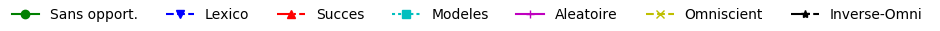
\includegraphics[width=\linewidth]{images/legende_mw.png}
	\end{subfigure}
	\caption{Comparaison sur tous les problèmes Moré-Wild avec \CS, avec opportunisme simple.}
	\label{fig:csmw}
\end{figure}

Premièrement, dans la figure \ref{fig:csmw} on observe que la stratégie d'ordonnancement omnisciente semble bien remplir son objectif d'agir en tant que borne supérieure lorsque jumelée à l'opportunisme simple. Sa performance supérieure est indéniable, pouvant aller jusqu'à 50\% de plus de problèmes résolus à précision $\tau = 10^{-3}$ que son plus proche adversaire, pour un abscisse donné.

Il en va de même pour la stratégie inverse-omnisciente. Sa performance tel qu'observée indique  que l'utilisation de la stratégie opportuniste peut être nuisible à la résolution de l'algorithme.
  
Les stratégies d'ordonnancement lexicographique, aléatoire, en direction du dernier succès et utilisant les modèles quadratiques sont des stratégies dites réalisables, contrairement aux stratégies de comparaison. Les stratégies réalisables les plus performantes sont les stratégies aléatoires et guidés par les modèles. Les profils de données montrent qu'elles sont de performances comparables. On remarque que, pour cet algorithme, seul la stratégie d'ordonnancement aléatoire contient des résolutions qui diffèrent selon la germe aléatoire, ce qui confère au profil un aspect beaucoup plus lisse. La courbe représentant l'ordonnancement guidé par modèle, contrairement à la courbe aléatoire, pourrait être améliorée avec des modèles plus représentatifs de la fonction qu'un modèle quadratique, tel qu'élaboré pour NOMAD dans~\cite{TaAuLedKo2018}.
  
Malgré que la stratégie en fonction du dernier succès soit plus raffinée que la stratégie aléatoire, elle ne prendra avantage de la forme du problème que si celui-ci n'est pas composé de plusieurs minimums locaux et de points de selle. On pourrait conclure que l'ensemble de problèmes utilisé ici possède une proportion de problèmes dont la structure n'est pas idéale pour un ordonnancement basé uniquement sur le succès précédent. La stratégie fonctionne relativement bien si comparée à la méthode non-opportuniste et présente une option déterministe peu raffinée.
 
La stratégie lexicographique n'est pas comparable en terme de performance. Elle pousse l'algorithme à épuiser ses sources de directions de descente une par une. Au fil des évaluations, si le point initial est un maximum, les directions de descente déjà épuisées seront évaluées en début de sonde, et celles prometteuses seront toujours à la fin de la liste, ce qui aura pour effet de décaler les succès de plus en plus au cours du déroulement de l'algorithme. On voit dans la stratégie lexicographique un exemple de mauvaise utilisation de la stratégie opportuniste.   

La stratégie non-opportuniste nécessite $n$ fois plus d'évaluation que la stratégie omnisciente pour chaque étape fructueuse de sonde et converge assurément vers le même points si la fonction n'incorpore pas d'aspects aléatoires. On peut observer quantitativement l'effet des évaluations supplémentaires nécessités par la méthode sans opportunisme. Celle-ci n'est certainement pas gage de résolution optimale, puisque les stratégies d'ordonnancement aléatoires et guidé par modèles y sont en tout point supérieur. Cependant, on remarque que sa courbe est d'avantage linéaire, ce qui indique que pour un grand budget d'évaluations, elle consiste en un choix sure. 

\begin{figure}[!htb]\label{fig:cs_mw_q}
	\centering
	\begin{subfigure}{0.43\textwidth}
		\includegraphics[width=\linewidth]{images/data_c_TOUS_1E-3secsuc_log.png}
		\label{fig:data_c_TOUS_1E-3secsuc_log}
	\end{subfigure}%\hspace*{\fill}
	\begin{subfigure}{0.43\textwidth}
		\includegraphics[width=\linewidth]{images/data_c_TOUS_1E-7secsuc_log.png}
		\label{fig:data_c_TOUS_1E-7secsuc_log}
	\end{subfigure}
	\smallskip
	\begin{subfigure}{0.95\textwidth}
		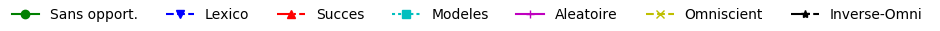
\includegraphics[width=\linewidth]{images/legende_mw.png}
	\end{subfigure}
	\caption{Comparaison sur tous les problèmes Moré-Wild avec \CS, avec opportunisme au $p=2^{text{ème}}$ succès.}
\end{figure}

La figure~\ref{fig:cs_mw_q} montre que tous les profils semblent avoir le même comportement. Par ailleurs, le profil de la stratégie omnisciente est indiscernable. Ceci est du au fait que la mécanique derrière le paramètre \texttt{OPPORTUNISTIC\_MIN\_NB\_SUCCES} impose que le deuxième succès trouvé soit par rapport au premier. Ainsi, la sonde est arrêtée seulement si $f(\tau_2) < f(\tau_1) < f(x^*)$, avec $\tau_1 \in P^k$ le premier succès obtenu dans la séquence d'évaluations de la sonde et $\tau_2$ le deuxième succès. C'est pourquoi chaque courbe est très similaire à la courbe de la sonde complete. Ceci explique aussi pourquoi il est impossible d'observer la courbe de l'ordonnancement omniscient, compte tenu que celle-ci est jointe à la courbe de l'algorithme sans opportunisme. En effet, si la première évaluation est le meilleur succès possible, alors il sera impossible d'en trouver un deuxième satisfaisant le critère d'opportunisme du paramètre.

\begin{figure}[!htb]
	\centering
	\begin{subfigure}{0.43\textwidth}
		\includegraphics[width=\linewidth]{images/data_c_TOUS_1E-3mineval_log.png}
		\label{fig:data_c_TOUS_1E-3mineval_log}
	\end{subfigure}%\hspace*{\fill}
	\begin{subfigure}{0.43\textwidth}
		\includegraphics[width=\linewidth]{images/data_c_TOUS_1E-7mineval_log.png}
		\label{fig:data_c_TOUS_1E-7mineval_log}
	\end{subfigure}
	\smallskip
	\begin{subfigure}{0.95\textwidth}
		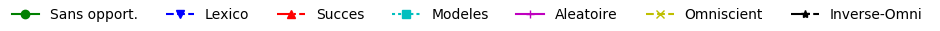
\includegraphics[width=\linewidth]{images/legende_mw.png}
	\end{subfigure}
	\caption{Comparaison sur tous les problèmes Moré-Wild avec \CS, avec minimum $q~=~\lceil\frac{n}{2}\rceil$ évaluations.} 
	\label{fig:cs_mw_p}
\end{figure} 
 
 
Dans la figure \ref{fig:cs_mw_p}, on observe le même ordre apparent entre les stratégies d'ordonnancement, ainsi que les mêmes tendances propre à chaque stratégie. Toutefois, on remarque aussi que les courbes sont rapprochées les unes avec les autres. La dominance de la stratégie omnisciente n'est pas aussi évidente que dans celle observable dans la figure~\ref{fig:csmw}. L'opportunisme avec un minimum de $p=\lceil\frac{n}{2}\rceil$ ne semble pas avoir le potentiel d'accélérer autant la résolution que l'opportunisme simple. La stratégie d'ordonnancement avec modèles semblent bénéficier des évaluations supplémentaires dans la mesure où elle semble être un peu supérieure à la stratégie aléatoire, contrairement à ce qui était observé à la figure \ref{fig:csmw}. 

En conclusion, on observe que la stratégie d'ordonnancement impacte fortement la performance d'une étape de sonde opportuniste. Les ordonnancement aléatoires et guidés par modèles sont ceux qui entraînent le plus grand gain possible. L'ordonnancement par la direction du dernier succès est aussi bénéfique mais dans une moindre mesure. La stratégie lexicographique nuit à la résolution de problèmes. On en conclu aussi qu'en utilisant le profil de données de l'algorithme sans opportunisme, on observe que l'opportunisme simple tel qu'existant dans NOMAD offre une meilleure possibilité d'accélérer la résolution de problèmes. La stratégie opportniste au $2^{\text{ème}}$ succès, tel qu'implémentée dans NOMAD, ne propose pas une alternative intéressante à l'opportunisme simple. La stratégie opportuniste avec un minimum de $\lceil\frac{n}{2}\rceil$ évaluations non plus, compte tenu que les tests démontrent qu'elle limite les gains en performances issus de l'utilisation de l'opportunisme.
\subsection{GPS}\label{sec:cgp}
La recherche par motifs généralisée est une version améliorée de la recherche par coordonnées. On s'attend à voir les mêmes impacts des stratégies opportunistes et la même hiérarchie entre les stratégies mais dans une mesure moins prononcée.
\begin{figure}[!htb]
	\centering
	\begin{subfigure}{0.43\textwidth}
		\includegraphics[width=\linewidth]{images/data_g_TOUS_1E-3og_log.png}
		\label{fig:data_g_TOUS_1E-3og_log}
	\end{subfigure}%\hspace*{\fill}
	\begin{subfigure}{0.43\textwidth}
		\includegraphics[width=\linewidth]{images/data_g_TOUS_1E-7og_log.png}
		\label{fig:data_g_TOUS_1E-7og_log}
	\end{subfigure}
	\smallskip
	\begin{subfigure}{0.95\textwidth}
		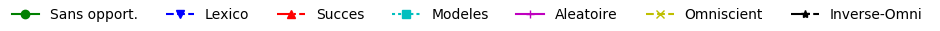
\includegraphics[width=\linewidth]{images/legende_mw.png}
	\end{subfigure}
	\caption{Comparaison sur tous les problèmes Moré-Wild avec \GPS, avec opportunisme simple.}
	\label{fig:gpsmw}
\end{figure}
À la figure~\ref{fig:gpsmw}, on remarque en effet que les courbes sont rapprochées les unes des autres. L'expansion du maillage permet d'éviter plusieurs étapes de sondes fructueuses, ce qui a pour effet de limiter l'impact possible de l'opportunisme. On remarque la même hiérarchie des stratégies observée avec l'opportunisme simple est présente, mais de façon moins prononcée. 

On observe toujours que la stratégie opportuniste surplombe les autres, mais avec \GPS elle est talonnée par la stratégie d'ordonnancement guidé par modèles. Il est moins évident avec \GPS qu'avec \CS de définir un classement des stratégies par performance, mais on peut affirmer que la stratégie lexicographique semble toujours nuire aux résolutions mais dans une moindre mesure. Les stratégies de la sonde complete, l'opportunisme avec ordonnancement aléatoire et avec ordonnancement selon la direction du dernier succès semblent avoir des performances très comparables. On observe principalement que l'écart entre la courbe de l'opportunisme omniscient et l'opportunisme inverse-omniscient n'est pas aussi importante qu'avec \CS. On reconnaît ainsi que l'opportunisme a un moins grand potentiel d'influence sur \GPS que sur \CS.

\begin{figure}[!htb]
	\centering
	\begin{subfigure}{0.43\textwidth}
		\includegraphics[width=\linewidth]{images/data_g_TOUS_1E-3secsuc_log.png}
		\label{fig:data_g_TOUS_1E-3secsuc_log}
	\end{subfigure}%\hspace*{\fill}
	\begin{subfigure}{0.43\textwidth}
		\includegraphics[width=\linewidth]{images/data_g_TOUS_1E-7secsuc_log.png}
		\label{fig:data_g_TOUS_1E-7secsuc_log}
	\end{subfigure}
	\smallskip
	\begin{subfigure}{0.95\textwidth}
		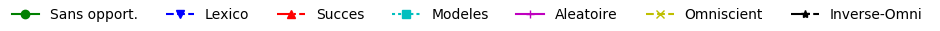
\includegraphics[width=\linewidth]{images/legende_mw.png}
	\end{subfigure}
	\caption{Comparaison sur tous les problèmes Moré-Wild avec \GPS, avec opportunisme au $p=2^{\text{ème}}$ succès.}
	\label{fig:gpsmwsecsuc}
\end{figure}

La figure~\ref{fig:gpsmwsecsuc} révèle que la tendance observée pour \GPS avec l'opportunisme simple se transfère dans celle observée pour l'opportunisme au deuxième succès. On voit que les profils sont difficilement dissociables les uns des autres, ce qui concrétise l'idée que l'opportunisme au deuxième succès tel qu'implémenté dans NOMAD porte l'algorithme à se comporter de façon non-opportuniste.

\begin{figure}[!htb]
	\centering
	\begin{subfigure}{0.43\textwidth}
		\includegraphics[width=\linewidth]{images/data_g_TOUS_1E-3mineval_log.png}
		\label{fig:data_g_TOUS_1E-3mineval_log}
	\end{subfigure}%\hspace*{\fill}
	\begin{subfigure}{0.43\textwidth}
		\includegraphics[width=\linewidth]{images/data_g_TOUS_1E-7mineval_log.png}
		\label{fig:data_g_TOUS_1E-7mineval_log}
	\end{subfigure}
	\smallskip
	\begin{subfigure}{0.95\textwidth}
		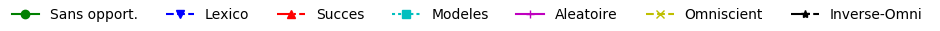
\includegraphics[width=\linewidth]{images/legende_mw.png}
	\end{subfigure}
	\caption{Comparaison sur tous les problèmes Moré-Wild avec \GPS, avec minimum $q~=~\lceil\frac{n}{2}\rceil$ évaluations.} 
	\label{fig:gps_mw_mineval}
\end{figure} 

La figure~\ref{fig:gps_mw_mineval} présente des résultats similaires à la figure~\ref{fig:gpsmw} mais en plus condensé. Il s'agit d'observations similaires que celles qui avaient été faites pour \CS. Il semble y avoir toutefois une bonne performance de la stratégie d'ordonnancement avec modèles, qui semble bénéficier des évaluations supplémentaires lui permettant de raffiner les modèles nécessaires à l'ordonnancement.

En conclusion, l'opportunisme a un effet moins important sur \GPS que sur \CS. Les stratégies d'ordonnancement préférables est la stratégie d'ordonnancement par modèle, quoique la stratégie aléatoire semble très performante pour son niveau de complexité. L'ordonnancement au $p=2^{\text{ème}}$ succès et l'ordonnancement avec $q=\lceil\frac{n}{2}\rceil$ semble rapprocher l'algorithme à sa version non-opportuniste, et ce peu importe la stratégie d'ordonnancement employée.
\subsection{MADS}\label{sec:cma}
\MADS est un algorithme qui génère un plus grand nombre de directions que \GPS, en plus de pouvoir nécessité moins d'évaluations pour ses étapes infructueuses. Puisque la convergence est plus rapide, les étapes de sondes qui sont des succès seront plus importante dans la vitesse de résolution.
\begin{figure}[!htb]
	\centering
	\begin{subfigure}{0.43\textwidth}
		\includegraphics[width=\linewidth]{images/data_m_TOUS_1E-3og_log.png}
		\label{fig:data_m_TOUS_1E-3og_log}
	\end{subfigure}%\hspace*{\fill}
	\begin{subfigure}{0.43\textwidth}
		\includegraphics[width=\linewidth]{images/data_m_TOUS_1E-7og_log.png}
		\label{fig:data_m_TOUS_1E-7og_log}
	\end{subfigure}
	\smallskip
	\begin{subfigure}{0.95\textwidth}
		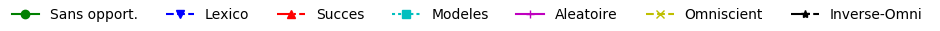
\includegraphics[width=\linewidth]{images/legende_mw.png}
	\end{subfigure}
	\caption{Comparaison sur tous les problèmes Moré-Wild avec \MADS, avec opportunisme simple.}
	\label{fig:mads_mw}
\end{figure}
On constate à la figure~\ref{fig:mads_mw} que l'impact de la stratégie opportuniste est plus important sur \MADS que sur \GPS. La stratégie omnisciente indique qu'un gain en performance est possible avec \MADS beaucoup plus qu'avec \GPS, et ce même à haute précision. 

Outre le gain possible, la figure montre que la stratégie d'ordonnancement avec modèles est la stratégie réalisable la plus fiable pour cet ensemble de problème. L'ordonnancement aléatoire et en fonction de la direction du dernier succès offrent une meilleure performance que la méthode sans-opportunisme. Celle-ci est comparable à la stratégie lexicographique. Toutes les stratégies réalisables offrent une performance similaire pour un budget de $10(n+1)$ à $100(n+1)$ évaluations, ce qui nous indique que, pour des budgets d'évaluations limités, l'importance de la stratégie d'ordonnancement, ou même de l'utilisation de l'opportunisme, peut être mise en doute. 

\begin{figure}[!htb]
	\centering
	\begin{subfigure}{0.43\textwidth}
		\includegraphics[width=\linewidth]{images/data_m_TOUS_1E-3secsuc_log.png}
		\label{fig:data_m_TOUS_1E-3secsuc_log}
	\end{subfigure}%\hspace*{\fill}
	\begin{subfigure}{0.43\textwidth}
		\includegraphics[width=\linewidth]{images/data_m_TOUS_1E-7secsuc_log.png}
		\label{fig:data_m_TOUS_1E-7secsuc_log}
	\end{subfigure}
	\smallskip
	\begin{subfigure}{0.95\textwidth}
		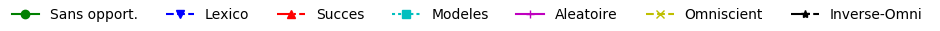
\includegraphics[width=\linewidth]{images/legende_mw.png}
	\end{subfigure}
	\caption{Comparaison sur tous les problèmes Moré-Wild avec \MADS, avec opportunisme au $p=2^{\text{ème}}$ succès.}
	\label{fig:mads_mw_secsuc}
\end{figure}

[je ne suis pas sur de comprendre ce qui se passe ici. la stratégie devrait se comporter comme précédemment. ]

\begin{figure}[!htb]
	\centering
	\begin{subfigure}{0.43\textwidth}
		\includegraphics[width=\linewidth]{images/data_m_TOUS_1E-3mineval_log.png}
		\label{fig:data_m_TOUS_1E-3mineval_log}
	\end{subfigure}%\hspace*{\fill}
	\begin{subfigure}{0.43\textwidth}
		\includegraphics[width=\linewidth]{images/data_m_TOUS_1E-7mineval_log.png}
		\label{fig:data_m_TOUS_1E-7mineval_log}
	\end{subfigure}
	\smallskip
	\begin{subfigure}{0.95\textwidth}
		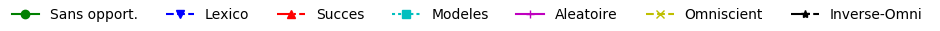
\includegraphics[width=\linewidth]{images/legende_mw.png}
	\end{subfigure}
	\caption{Comparaison sur tous les problèmes Moré-Wild avec \MADS, avec minimum $q~=~\lceil\frac{n}{2}\rceil$ évaluations.} 
	\label{fig:mads_mw_mineval}
\end{figure} 

La figure~\ref{fig:mads_mw_mineval} montre que l'oppotunisme avec au minimum $q~=~\lceil\frac{n}{2}\rceil$ évaluations n'est pas très différent de l'opportunisme simple, outre la performance diminuée de la stratégie omnisciente. L'apport de cette stratégie opportuniste est limitée mais encore une fois, on peut y percevoir que la stratégie utilisant les modèles pour l'ordonnancement bénéficie des évaluations supplémentaires. On peut aussi en comprendre que, pour \MADS avec opportunisme simple et une stratégie d'ordonnancement réalisable, les étapes de sondes comportent un nombre d'évaluations comparable à $\lceil\frac{n}{2}\rceil$, sans quoi l'allure des courbes ne seraient pas aussi similaires.

En conclusion, \MADS a d'avantage à gagner que \GPS à utiliser une stratégie opportuniste simple et une stratégie d'ordonnancement telle que l'ordonnancement à l'aide de modèles quadratique. Cette stratégie domine les stratégies aléatoires et en fonction de la direction du dernier succès, qui sont elles aussi des stratégies bénéfiques. La stratégie d'ordonnancement lexicographique n'est pas recommandée, compte tenu que la méthode sans opporutnisme semble avoir la même performance pour un comportement plus stable.

\subsection{\MADS par défaut}\label{sec:ctr}
Afin d'observer l'impact de l'opportunisme et le gain possible en performance possible, les problèmes de l'ensemble Moré-Wild sont résolus à l'aide de NOMAD avec ses paramètres par défaut. La stratégie lexicographique n'est pas représentée, compte tenu d'un conflit existant au sein de l'implémentation avec l'utilisation de modèles quadratiques en tant que \SEARCH.

\begin{figure}[!htb]
	\centering
	\begin{subfigure}{0.43\textwidth}
		\includegraphics[width=\linewidth]{images/data_t_TOUS_1E-3og_log.png}
		\label{fig:data_t_TOUS_1E-3og_log}
	\end{subfigure}%\hspace*{\fill}
	\begin{subfigure}{0.43\textwidth}
		\includegraphics[width=\linewidth]{images/data_t_TOUS_1E-7og_log.png}
		\label{fig:data_t_TOUS_1E-7og_log}
	\end{subfigure}
	\smallskip
	\begin{subfigure}{0.95\textwidth}
		\includegraphics[width=\linewidth]{images/legend_mw_wo_lexico.png}
	\end{subfigure}
	\caption{Comparaison sur tous les problèmes Moré-Wild avec \MADS par défaut de NOMAD, avec opportunisme simple.}
	\label{fig:true_mw}
\end{figure}

Dans la figure \ref{fig:true_mw}, on observe que le gain possible avec un ordonnancement parfait est réduit lorsque NOMAD est utilisé au meilleur de ses capacités. Seules les courbes des stratégies d'ordonnancement irréalisables de distinguent des autres. En observant la courbe omnisciente, on comprends que le gain possible est limité à un maximum de 15\% de problèmes pour un budget donné. Cependant, il est important rappeler que l'ensemble de problèmes Moré-Wild est un ensemble de problèmes analytiques non contraints peu représentatifs des problèmes encourus en optimisation de boîtes noires. Les figures pour NOMAD par défaut avec les deux autres types d'opportunisme sont omises, compte tenu de leur similarités avec la figure \ref{fig:true_mw}.

\subsection{\GSS}\label{sec:cgs} 
Les problèmes Moré-Wild sont résolus avec HOPSPACK, qui est par défaut opportuniste, avec les deux stratégies d'ordonnancement déjà implémentées à même le logiciel. Une mise à niveau a du être fournie à HOPSPACK, inspirée de~\cite{AuLedTr2014}, consistant en l'obtention de
	\[\Delta^0_j =  \begin{cases} 
	\frac{|x^0_j|}{10} & |x^0_j| \neq 0 \\
	1 & |x^0_j| = 0
	\end{cases}
	\]
où $\Delta_j^0$ est la $j^{\text{ème}}$ composante du pas initial, et $x^0_j$ la $j^{\text{ème}}$ composante du point de départ $x^0$. Seul l'opportunisme simple est implémenté dans HOPSPACK.
\begin{figure}[!htb]
	\centering
	\begin{subfigure}{0.43\textwidth}
		\includegraphics[width=\linewidth]{images/data_gss_TOUS_1E-3og_log.png}
		\label{fig:data_gss_TOUS_1E-3og_log}
	\end{subfigure}%\hspace*{\fill}
	\begin{subfigure}{0.43\textwidth}
		\includegraphics[width=\linewidth]{images/data_gss_TOUS_1E-7og_log.png}
		\label{fig:data_gss_TOUS_1E-7og_log}
	\end{subfigure}
	\smallskip
	\begin{subfigure}{0.95\textwidth}
		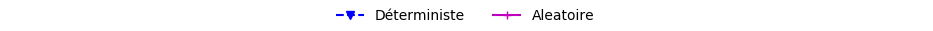
\includegraphics[width=\linewidth]{images/legende_gss.png}
	\end{subfigure}
	\caption{Comparaison sur tous les problèmes Moré-Wild avec \GSS avec opportunisme simple.}
	\label{fig:legende_gss}
\end{figure}
La figure~\ref{fig:legende_gss} nous permet d'observer la comparaison de deux stratégies d'ordonnancement présente dans une autre implémentation que NOMAD. On observe que la stratégie aléatoire est nettement supérieure à la stratégie déterministe de HOPSPACK. On observe ici directement l'impact qu'un choix d'ordonnancement déterministe peut avoir sur la résolution. La mise en valeur arbitraire de certaines directions tend à nuire à l'algorithme. Il est à noté que le paramètre par défaut de HOPSPACK quant à l'ordonnancement est l'ordonnancement déterministe. On en conclue que la supériorité de l'ordonnancement aléatoire quant à l'ordonnancement déterministe se transmet dans diverses implémentations, et que l'ordonnancement aléatoire se distingue comme un choix judicieux nécéssitant peu d'efforts.
\subsection{\imfil}\label{sec:cim}
L'implémentation utilisée de \imfil nécessite que l'utilisateur fournisse des bornes, duquel en découle une mise à l'échelle pour la résolution. Les problèmes Moré-Wild étant non bornés, des bornes arbitraires ont du être déterminées. Pour ce faire, on utilise
\begin{gather*}
	u_i = 10^{1+\lfloor\log(\max(|x_i^0|,|x_i^*|))\rfloor}\\
	l_i=-u_i
\end{gather*}
avec $u$ le vecteur des bornes supérieures, $l$ le vecteur des bornes inférieures, $x^0$ le point initial fourni avec le problème et $x^*$ la solution trouvée par l'algorithme \MADS par défaut de NOMAD sur le problème donné. Ainsi, on fournit à \imfil un domaine dont les limites sont une puissance de 10, centré en 0, symétrique et qui contient assurément le point de départ et la solution.
\begin{figure}[!htb]
	\centering
	\begin{subfigure}{0.43\textwidth}
		\includegraphics[width=\linewidth]{images/data_i_TOUS_1E-3OP_log.png}
	\end{subfigure}
	\begin{subfigure}{0.43\textwidth}
		\includegraphics[width=\linewidth]{images/data_i_TOUS_1E-7OP_log.png}
	\end{subfigure}
	\smallskip
	\begin{subfigure}{0.95\textwidth}
		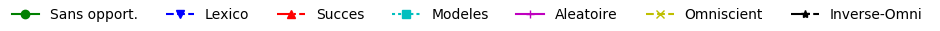
\includegraphics[width=\linewidth]{images/legende_mw.png}
	\end{subfigure}
	\caption{Comparaison sur tous les problèmes Moré-Wild avec \imfil avec opportunisme \textsf{op}}
	\label{fig:i_mw_op}
\end{figure}
À la figure \ref{fig:i_mw_op}, on observe que \imfil n'est pas en mesure de bénéficier pleinement de la stratégie opportuniste textsf{op}. On observe en premier lieu que le profil correspondant à la stratégie d'ordonnancement omnisciente offre un meilleur rendement que la méthode sans opporutnisme pour un certain budget, et ce à précision $\tau = 1E-3$ seulement. Le profil de l'ordonnancement négatif-omniscient se comporte de façon très similaire à la méthode sans opporutnisme. On explique ceci avec la nature de \imfil. Puisque la sonde opportuniste inverse-omnisciente permet l'évaluation d'un grand nombre de points, le \textsf{BLS} est effectué dans une direction comprenant plusieurs composantes non-nulles.  

Malgré que la stratégie d'ordonnancement omnisciente semble procurer un gain en performance à basse précision, on observe que les stratégies réalisables nuisent aux résolutions. Aucune stratégie n'est en mesure de se démarquer comme étant un choix intéressant pour l'algorithme. À haute précision $\tau = 1E-7$, on remarque que la version opportuniste de \imfil avec une stratégie d'ordonnancement réalisable n'est pas en mesure d'obtenir les solutions précises pour $50\%$ des problèmes seulement, comparativement à près de $80\%$ avec la méthode sans opporutnisme, ce qui témoigne que les meilleurs résultats $f^*$ proviennent en majorité de celles-ci.
\begin{figure}[!htb]
	\centering
	\begin{subfigure}{0.43\textwidth}
		\includegraphics[width=\linewidth]{images/data_i_TOUS_1E-3OD_log.png}
	\end{subfigure}
	\begin{subfigure}{0.43\textwidth}
		\includegraphics[width=\linewidth]{images/data_i_TOUS_1E-7OD_log.png}
	\end{subfigure}
	\smallskip
	\begin{subfigure}{0.95\textwidth}
		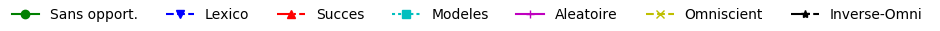
\includegraphics[width=\linewidth]{images/legende_mw.png}
	\end{subfigure}
	\caption{Comparaison sur tous les problèmes Moré-Wild avec \imfil avec opportunisme \textsf{od}}
	\label{fig:i_mw_od}
\end{figure}
La figure~\ref{fig:i_mw_od} témoigne de l'incompatibilité entre la stratégie opportuniste \textsf{op} et \imfil. La méthode sans opportunisme résout la meilleure proportion de problème, peu importe le budget alloué. Les stratégies omniscientes et inverse-omnisciente ne sont pas discernables des autres stratégies. À haute précision, on remarque qu'aucune stratégie d'ordonnancement ne permet de d'obtenir un rendement comparable à la méthode sans opporutnisme.

L'arrêt de la sonde du stencil directement après la détection d'un candidat amenant un succès semble avoir un effet plus prononcé que l'opportunisme après minimum$\lceil \frac{n}{2}\rceil$, qui semble se comporter comme une version moins performante de \imfil avec méthode sans opporutnisme. En conclusion, l'opportunisme implanté dans \imfil n'est pas bénéfique à la méthode, tel que prédit par son auteur, puisqu'aucune combinaison de stratégie opportuniste et de stratégie d'ordonnancement réaliste n'est en mesure d'accélérer les résolutions.
\section{Comparaison des stratégies d'ordonnancement sur les problèmes contraints}\label{sec:com2}
Pour l'ensemble de problèmes contraints, les profils de données sont tracés avec les seuils de tolérance $\tau = 10^{-1}$ et $\tau = 10^{-3}$, puisque les solutions trouvées par les algorithmes n'ont pas la même reproductibilité que les problèmes Moré-Wild. Les paramètres $p$ et $q$ des stratégies opportunistes des définitions~\ref{def:oppemesucces} et~\ref{def:opmineval} sont respectivement $p=2$ et $q = \lceil\frac{n}{2}\rceil$, à l'instar des comparaisons de la section~\ref{sec:com}. Les profils de données pour ces stratégies opportunistes sont fournis à l'annexe~\ref{ann:A}. Seuls les algorithmes implémentés dans NOMAD, soit \CS, \GPS et \MADS, pouvant gérer les contraintes à l'aide de la barrière progressive, sont testés sur ces problèmes. Chaque point initial utilisé est un point irréalisable.
\subsection{\CS et \GPS}\label{sec:cs_gps_const}
Les algorithmes \CS et \GPS sont jumelés dans cette section en vertu des résultats similaires que les profils de données permettent d'observer.

\begin{figure}[!htb]
	\centering
	\begin{subfigure}{0.43\textwidth}
		\includegraphics[width=\linewidth]{images/data_c_CONSTRAINED_1E-1OG_log.png}
	\end{subfigure}%\hspace*{\fill}
	\begin{subfigure}{0.43\textwidth}
		\includegraphics[width=\linewidth]{images/data_c_CONSTRAINED_1E-3OG_log.png}
	\end{subfigure}
	\smallskip
	\begin{subfigure}{0.95\textwidth}
		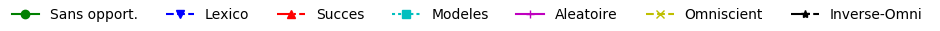
\includegraphics[width=\linewidth]{images/legende_mw.png}
	\end{subfigure}
	\caption{Comparaison sur tous les problèmes contraints avec \CS avec opportunisme simple.}
	\label{fig:cs_const_og}
\end{figure}
\begin{figure}[!htb]
	\centering
	\begin{subfigure}{0.43\textwidth}
		\includegraphics[width=\linewidth]{images/data_g_CONSTRAINED_1E-1OG_log.png}
	\end{subfigure}%\hspace*{\fill}
	\begin{subfigure}{0.43\textwidth}
		\includegraphics[width=\linewidth]{images/data_g_CONSTRAINED_1E-3OG_log.png}
	\end{subfigure}
	\smallskip
	\begin{subfigure}{0.95\textwidth}
		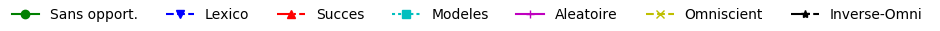
\includegraphics[width=\linewidth]{images/legende_mw.png}
	\end{subfigure}
	\caption{Comparaison sur tous les problèmes contraints avec \GPS avec opportunisme simple.}
	\label{fig:gps_const_og}
\end{figure}

Premièrement, les figure~\ref{fig:cs_const_og} et~\ref{fig:gps_const_og} montrent que l'ensemble de problèmes utilisés est trop petit pour obtenir des courbes lisses. La tendance générale est qu'aucune stratégie d'ordonnancement jumelée à l'opportunisme simple pour \CS et \GPS n'est en mesure de se démarquer comme celle pouvant potentiellement apporter la meilleure amélioration. Cependant, en distinguant le profil correspondant à la méthode sans opportunisme à précision $\tau = 1E-1$, on remarque que celui-ci se trouve sous les courbes opportunistes, et ce pour tout budget d'évaluation. Ces observations sont valables pour les courbes des autres stratégies opportunistes, figurant sur les  figures~\ref{fig:cs_const_secsuc},~\ref{fig:cs_const_mineval},\ref{fig:gps_const_secsuc} et~\ref{fig:gps_const_mineval}  de l'annexe \ref{ann:A}.

On en conclu que l'opportunisme simple est une pratique qui impacte positivement la résolution de problèmes contraints, sans qu'aucune stratégie d'ordonnancement ne soit favorisé.
\subsection{\MADS}
 \smallskip\hfill
\begin{figure}[!htb]
	\centering
	\begin{subfigure}{0.43\textwidth}
		\includegraphics[width=\linewidth]{images/data_m_CONSTRAINED_1E-1OG_log.png}
	\end{subfigure}%\hspace*{\fill}
	\begin{subfigure}{0.43\textwidth}
		\includegraphics[width=\linewidth]{images/data_m_CONSTRAINED_1E-3OG_log.png}
	\end{subfigure}
	\smallskip
	\begin{subfigure}{0.95\textwidth}
		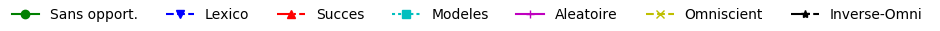
\includegraphics[width=\linewidth]{images/legende_mw.png}
	\end{subfigure}
	\caption{Comparaison sur tous les problèmes contraints avec \MADS avec opportunisme simple.}
	\label{fig:mads_const_og}
\end{figure}
La figure~\ref{fig:mads_const_og} permet d'observer une plus grande hiérarchie des stratégie d'ordonnancement qu'à la section~\ref{sec:cs_gps_const}. Les courbes sont plus lisses en vertu de la génération pseudo-aléatoire de directions possible avec \MADS, contrairement à \CS et \GPS, pour lesquels les résolutions sont parfaitement reproductibles indépendamment du germe aléatoire.

L'ordonnancement omniscient jumelé à l'opportunisme simple semble offrir une nette amélioration de l'algorithme \MADS en situation de barrière progressive. La performance de l'ordonnancement inverse-omniscient, quant à lui, démontre que l'intuition sur une mauvaise stratégie d'ordonnancement est toujours valide pour les problèmes contraints.

Les stratégies d'ordonnancement réalisables sont cependant de performance comparables avec la méthode sans opportunisme. La stratégie aléatoire et la stratégie lexicographique semblent nuire à l'algorithme. Les autres stratégies opportunistes ne semblent pas avoir le même effet sur la sonde, tel que les figures~\ref{fig:mads_const_secsuc} et~\ref{fig:mads_const_mineval} en témoignent. On en conclu qu'un gain en performance serait envisageable avec l'implémentation d'un ordonnancement guidé par un outil plus élaboré que les modèles quadratiques, mais que dans l'état actuel, ceux-ci permettent à l'opportunisme de ne pas nuire à la sonde de \MADS.
\subsection{\MADS par défaut}
\begin{figure}[!htb]
	\centering
	\begin{subfigure}{0.43\textwidth}
		\includegraphics[width=\linewidth]{images/data_t_CONSTRAINED_1E-1OG_log.png}
	\end{subfigure}%\hspace*{\fill}
	\begin{subfigure}{0.43\textwidth}
		\includegraphics[width=\linewidth]{images/data_t_CONSTRAINED_1E-3OG_log.png}
	\end{subfigure}
	\smallskip
	\begin{subfigure}{0.95\textwidth}
		\includegraphics[width=\linewidth]{images/legend_mw_wo_lexico.png}
	\end{subfigure}
	\caption{Comparaison sur tous les problèmes contraints avec \MADS par défaut de NOMAD avec opportunisme simple.}
	\label{fig:t_const_og}
\end{figure}
La figure~\ref{fig:t_const_og} montre que l'opportunisme a peu d'effet si on utilise \MADS par défaut de NOMAD. Les spécificités de \textsf{OrthoMADS} ainsi que l'influence d'une étape de \SEARCH noient l'impact de l'opportunisme sur cet ensemble de problème. Cependant, on remarque que le profil correspondant à l'ordonnancement inverse-omniscient nuit quelque peu les résolutions de problèmes, notamment au niveau de la proportion de problèmes résolus avec une précision de $\tau = 1E-3$. C'est avec cette précision qu'on observe que l'ordonnancement guidé par modèles semblent bénéficier à l'algorithme. 
\section{Comparaison des stratégies d'ordonnancement sur STYRENE}\label{sec:com3}
Les algorithmes étudiés sont limités à \MADS et à \MADS par défaut de NOMAD, en raison de la reproductibilité présente dans \CS et \GPS. Les stratégies d'ordonnancement sont comparées à l'aide de graphes de convergence, dans lesquels les courbes correspondantes aux stratégies omniscientes et inverse-omnisciente sont présente. Avec celles-ci figure la courbe correspondante à une stratégie comparée, de façon à observer la performance de cette stratégie relativement à la performance des stratégies de comparaison. Le point de départ des résolutions est irréalisable et déterminé suite à un échantillonnage du domaine de la boîte noire.
\subsection{\MADS}
\label{sec:sty_mads}
\begin{figure}[!htb]
	\centering
	\begin{subfigure}{0.43\textwidth}
		\includegraphics[width=\linewidth]{images/conv_mog_STYRENEX0_Omniscient_Inverse-Omni_no.png}
	\end{subfigure}
	\hspace*{\fill}
	\smallskip
	\begin{subfigure}{0.43\textwidth}
		\includegraphics[width=\linewidth]{images/conv_mog_STYRENEX0_Omniscient_Inverse-Omni_Lexicographique.png}
	\end{subfigure}%\hspace*{\fill}
	\begin{subfigure}{0.43\textwidth}
		\includegraphics[width=\linewidth]{images/conv_mog_STYRENEX0_Omniscient_Inverse-Omni_Aleatoire.png}
	\end{subfigure}
	\caption{Comparaison sur STYRENE avec \MADS et opportunisme simple, sonde complète, stratégie lexicographique et stratégie aléatoire.}
	\label{fig:m_styrene_1}
\end{figure}
Premièrement, le premier graphe de convergence de figure~\ref{fig:m_styrene_1} présente les courbes des stratégies de comparaison ainsi que la sonde complète. On observe que la convergence est significativement plus rapide avec la stratégie omnisciente qu'avec la stratégie inverse-omnisciente. De plus, on observe que la solution vers laquelle la stratégie omnisciente converge est un optimum beaucoup plus satisfaisant que celui obtenu par la stratégie inverse-omnisciente. La sonde complète a un comportement qui se rapproche d'avantage à celui de la stratégie inverse-omnisciente. Il s'agit d'une indication de la performance de la barrière progressive jumelée à la stratégie omnisciente, pour laquelle la mise a jour de $x^{\inf}$ est effectuée en admettant le point ayant la plus petite violation de contrainte. Inversement, l'algorithme de la barrière progressive de la sonde complète mets à jour $x^{\inf} \leftarrow t$, avec $t\in \arg \min{(T)}$ et $h(t)<h_{\max}$, où $T$ est l'ensemble des points non-dominés. Il en résulte que le premier point réalisable n'est pas le même.

La vitesse de résolution de la stratégie lexicographique s'apparente à celle de la stratégie inverse-omnisciente. Cependant, on remarque une certaines proportion de courbes convergeant vers une solution intermédiaires entre la solution de la sonde complète et celle de la stratégie omnisciente.

La stratégie aléatoire semble apporter une amélioration de performance en comparaison avec la sonde complète. La vitesse de résolution est similaire, mais la qualité de la solution obtenue est plus souvent semblable à celle obtenue avec la stratégie omnisciente.

\begin{figure}[!htb]
	\centering
	\begin{subfigure}{0.43\textwidth}
		\includegraphics[width=\linewidth]{images/conv_mog_STYRENEX0_Omniscient_Inverse-Omni_Succes.png}
	\end{subfigure}%\hspace*{\fill}
	\begin{subfigure}{0.43\textwidth}
		\includegraphics[width=\linewidth]{images/conv_mog_STYRENEX0_Omniscient_Inverse-Omni_Modeles.png}
	\end{subfigure}
	\caption{Comparaison sur STYRENE avec \MADS et opportunisme simple, stratégie avec direction du dernier succès et stratégie guidée par modèles.}
	\label{fig:m_styrene_2}
\end{figure}

La stratégie d'ordonnancement avec la direction du dernier succès ne permet pas à l'algorithme de converger vers la solution optimale déterminée avec la stratégie omnisciente, tel qu'observer sur la figure~\ref{fig:m_styrene_2}. Il en est de même pour la stratégie avec modèles. La fonction objectif et les contraintes de la boîte noire STYRENE sont difficilement modélisables à l'aide de fonctions quadratiques. Une fonction substitut plus représentative pourrait permettre à la solution de se rapprocher de la courbe omnisciente. Cependant, la vitesse de résolution pour la stratégie avec modèles plus grande qu'avec la stratégie de la direction du dernier succès.

Avec l'étape de sonde seule de \MADS, l'influence de la stratégie d'ordonnancement est importante pour la qualité de la solution obtenue et la vitesse de résolution. La stratégie lexicographique ralenti la résolution, mais son aspect quasi-aléatoire peut entraîner l'algorithme vers une meilleure solution. La stratégie aléatoire présente une vitesse de résolution significativement plus rapide que la stratégie lexicographique mais semblable à la sonde complète. Cependant, son aspect aléatoire peut permettre à l'algorithme de converger vers une meilleure solution. La stratégie de la direction de succès mène à la même solution que la sonde complète avec un léger gain en vitesse de résolution. La stratégie utilisant les modèles semble celle qui amène le meilleur gain en vitesse de résolution. Par contre, la solution vers laquelle $80\%$ résolutions converge n'est pas une amélioration quant à la sonde complète. Puisque le point de départ $x^0$ est irréalisable, on en conclu que la détermination du $x^{\inf}$ à chaque itération à un effet important sur la qualité de la solution obtenue, et qu'aucune stratégie réaliste utilisée ici ne permet d'ordonnancer les points de l'ensemble $P^k$ de façon à mettre de l'avant le meilleur candidat pour $x^{\inf}$.

\subsection{\MADS par défaut}
Il est à noter que la stratégie lexicographique n'est pas utilisée pour les comparaisons avec étape de \SEARCH. 
\begin{figure}[!htb]
	\centering
	\begin{subfigure}{0.43\textwidth}
		\includegraphics[width=\linewidth]{images/conv_tog_STYRENEX0_Omniscient_Inverse-Omni_no.png}
	\end{subfigure}%\hspace*{\fill}
	\begin{subfigure}{0.43\textwidth}
		\includegraphics[width=\linewidth]{images/conv_tog_STYRENEX0_Omniscient_Inverse-Omni_Aleatoire.png}
	\end{subfigure}
	\caption{Comparaison sur STYRENE avec \MADS par défaut et opportunisme simple, sonde complète et stratégie aléatoire.}
	\label{fig:t_styrene_1}
\end{figure}
Dans la figure~\ref{tab:t_styrene_1}, on remarque que la sonde complète converge vers la même solution que les stratégies de comparaison. La vitesse de résolution de la sonde complète est moins satisfaisante que celle de l'ordonnancement omniscient. La différence est beaucoup moins grande que celle observée avec \MADS. Les courbes de la stratégie aléatoire montrent que parfois la vitesse est supérieure à la sonde complète, parfois inférieure. Elles convergent en majorité vers la même solution.

\begin{figure}[!htb]
	\centering
	\begin{subfigure}{0.43\textwidth}
		\includegraphics[width=\linewidth]{images/conv_tog_STYRENEX0_Omniscient_Inverse-Omni_Succes.png}
	\end{subfigure}%\hspace*{\fill}
	\begin{subfigure}{0.43\textwidth}
		\includegraphics[width=\linewidth]{images/conv_tog_STYRENEX0_Omniscient_Inverse-Omni_Modeles.png}
	\end{subfigure}
	\caption{Comparaison sur STYRENE avec \MADS par défaut et opportunisme simple, stratégie avec direction du dernier succès et stratégie guidée par modèles.}
	\label{fig:t_styrene_2}
\end{figure}

La stratégie avec de la direction du dernier succès présente une performance intéressante. Jumelée avec l'étape de \SEARCH de \MADS par défaut, on observe que la stratégie a une performance similaire à celle de l'ordonnancement par modèles. L'ordonnancement guidé par modèles n'est pas aussi performant en présence de \SEARCH. Une mauvaise géométrie de points pour l'interpolation issue de la détermination de points seulement par les modèles peut être à l'origine de cette baisse d'impact.

Les impacts des stratégies d'ordonnancement sur STYRENE sont moins prononcés qu'avec \MADS sans \SEARCH de la section~\ref{sec:sty_mads}. Les solutions trouvées sont plus robustes avec la \SEARCH et l'ordonnancement influence en général seulement la vitesse de résolution. La stratégie d'ordonnancement utilisant la direction du dernier succès offre le meilleur rendement, mais l'impacte de l'opportunisme jumelé à la \SEARCH reste minime.